\subsection{Wellendiskussion}
\label{sec:wellen:diskussionwellenform}

Wie bereits ersichtlich, wechselt die Welle ihre Form bei den jeweiligen 
Nullstellen des Profils.

Es stellt sich heraus, dass die L"osung der Titelgleichung eng mit der 
gefundenen L"osung der Gleichung (\ref{eq:wellen:lineareDGL}) verwandt ist. So 
k"onnen die L"osungen des Parabelprofils als verschiedene $c$ Werte der 
linearen Differentialgleichung verstanden werden, welche dann in die 
L"osungsgleichung (\ref{eq:wellen:loesunglinearedgl}) eingesetzt werden 
k"onnen. Daraus ergibt es also f"ur negative Profill"osungen eine Kombination 
aus den hyperbolischen Funktionen $\sinh$ und $\cosh$ und f"ur positive eine 
Kombination aus $\sin$ und $\cos$.

\begin{figure}
	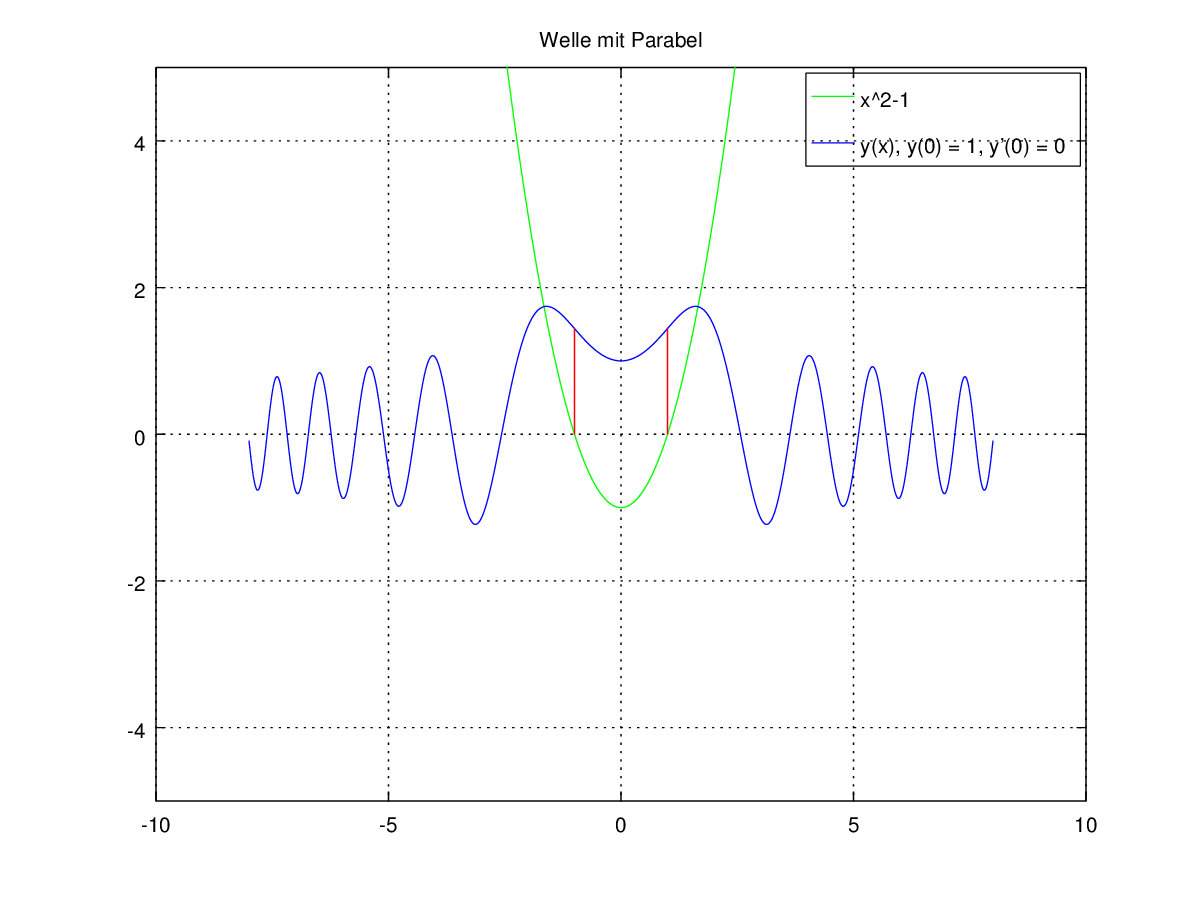
\includegraphics[scale=0.35]{./wellen/images/varc/cneg1.png}
	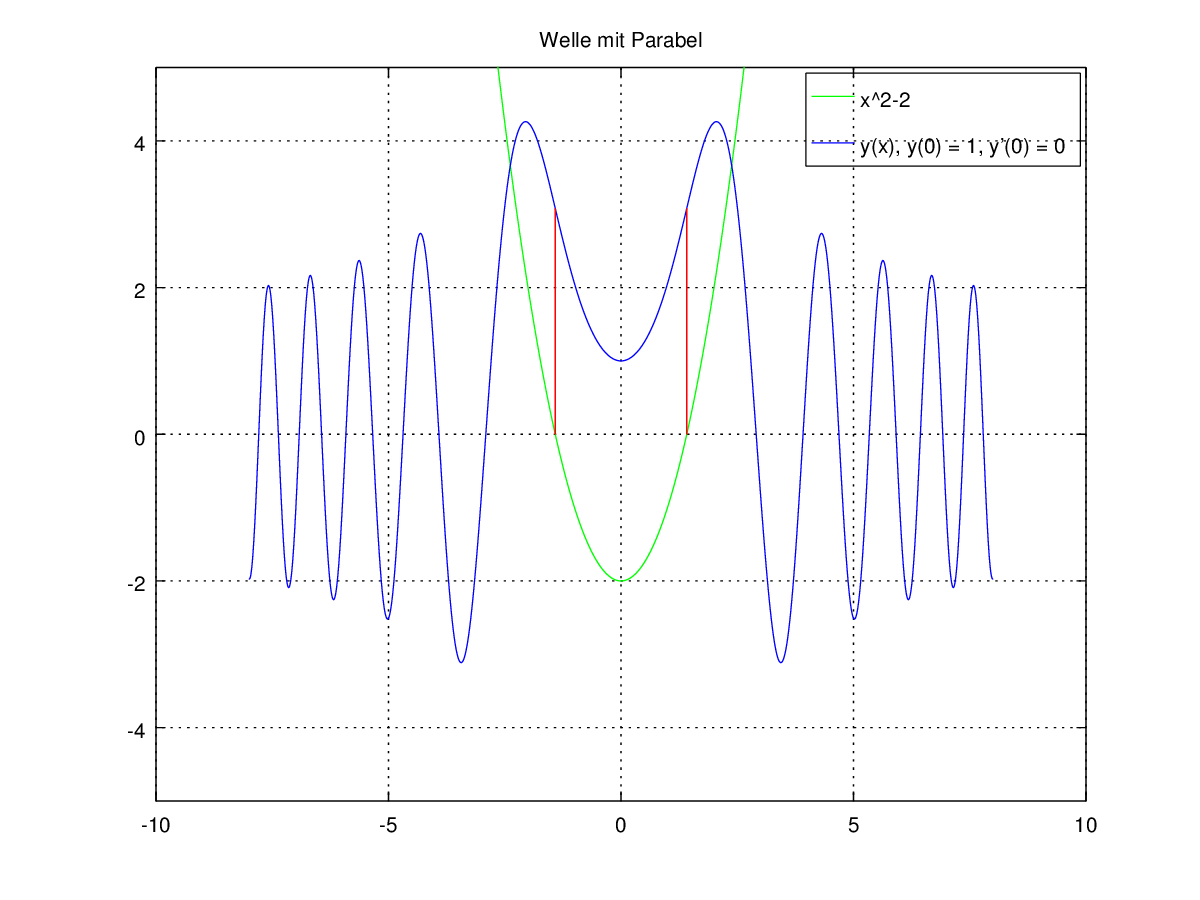
\includegraphics[scale=0.35]{./wellen/images/varc/cneg2.png}
	\caption{Wellenform mit unterschiedlichen $c$ Werten}
	\label{fig:wellen:variablec}
\end{figure}

\begin{figure}
	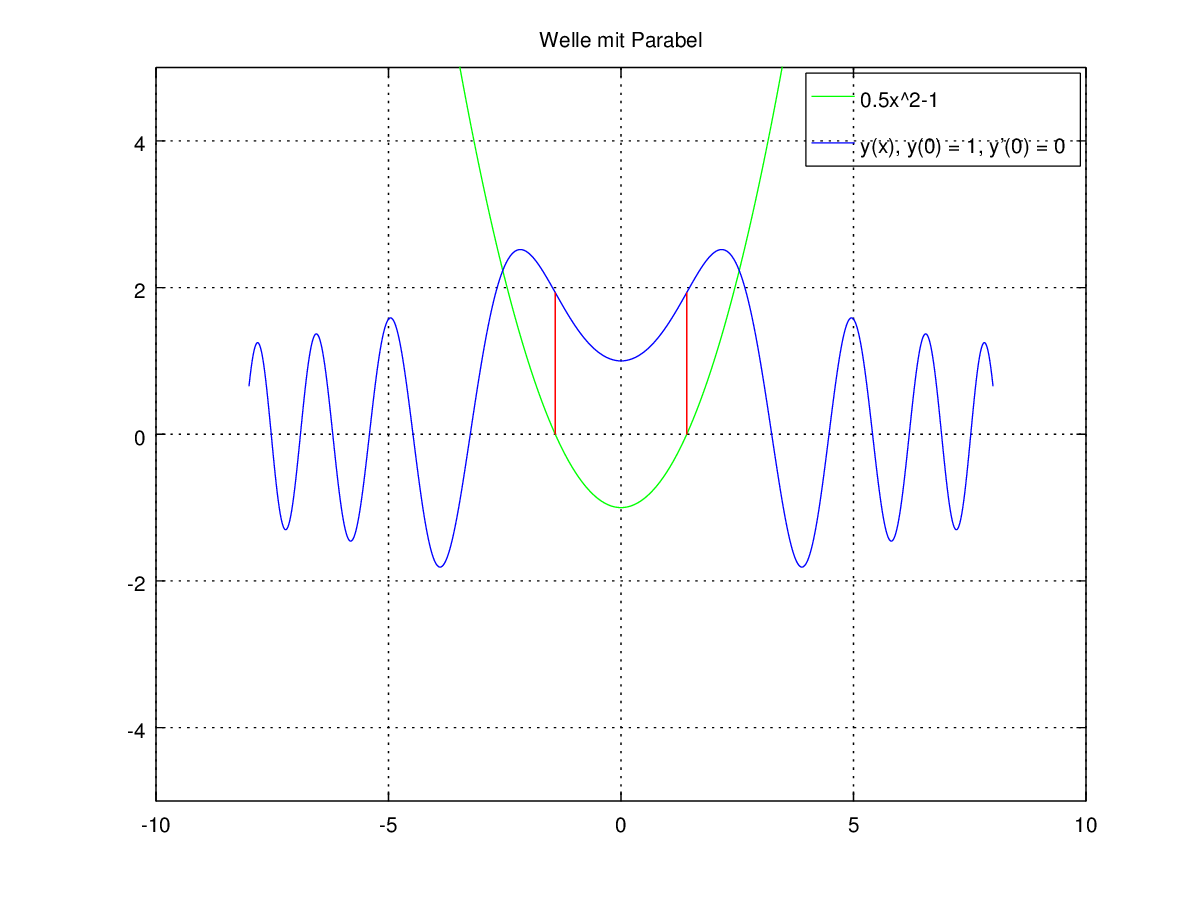
\includegraphics[scale=0.35]{./wellen/images/vara/ahalbe.png}
	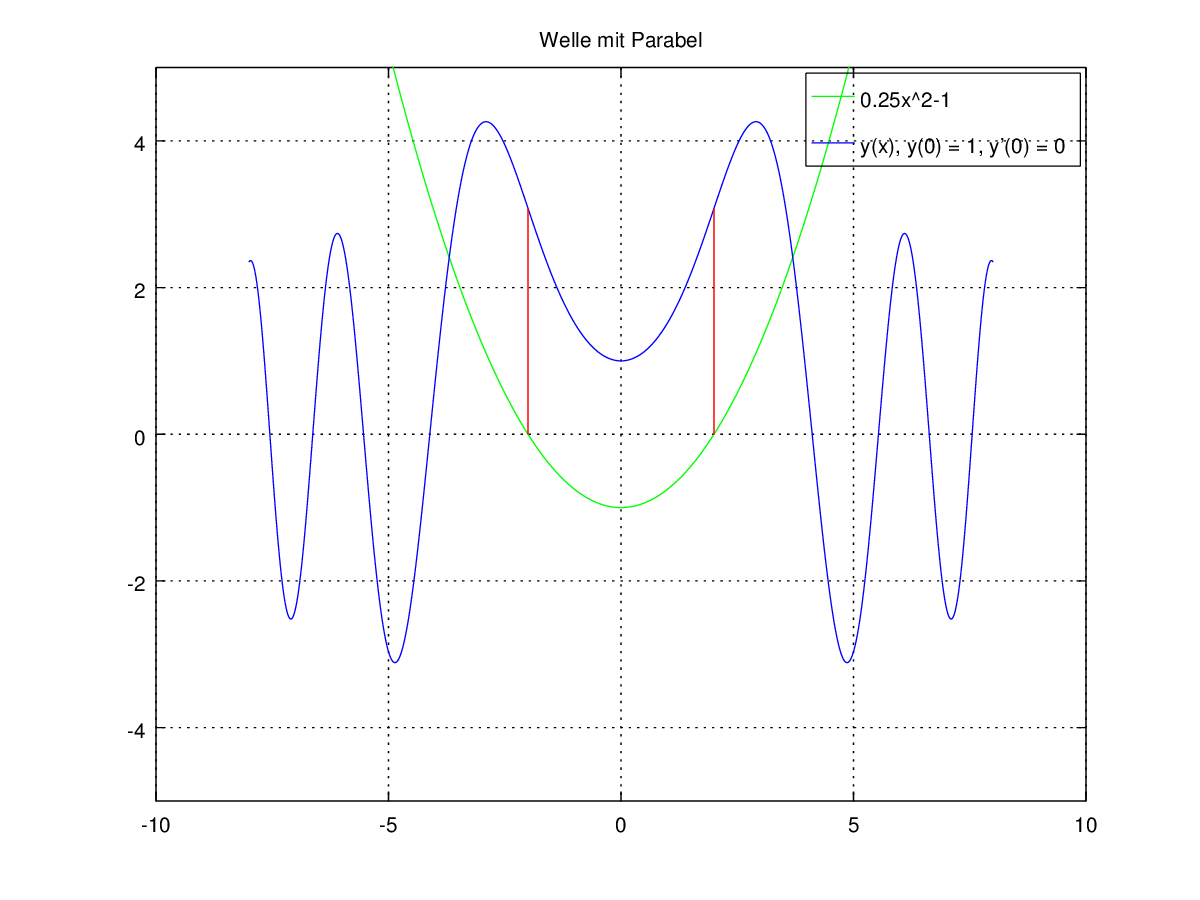
\includegraphics[scale=0.35]{./wellen/images/vara/aviertel.png}
	\caption{Wellenform bei unterschiedlichen $a$ Werten}
	\label{fig:wellen:variablea}
\end{figure}

Obwohl die Wellenformen bei variablem $c$ (Abbildung 
\ref{fig:wellen:variablec}) und $a$ (Abbildung \ref{fig:wellen:variablea}) 
alle "ahnlich sind, stellen wir fest, dass es bei den 
jeweiligen Nullstellen des Profiles eine gr"ossere Ver"anderung gibt.
